\section{Procedimiento}
Lorem ipsum dolor sit amet, consectetur adipiscing elit. Quisque at nisl sed quam fermentum ultrices id nec turpis. Donec et est nulla. Donec porttitor, mi vel aliquet fringilla, neque lacus aliquam ligula, non laoreet felis purus at ipsum. Quisque at gravida tortor. Donec id nisi ligula. Vivamus ornare quis nibh ut bibendum. Mauris pulvinar risus risus, eu luctus ligula tincidunt vitae. Nunc sit amet placerat nulla, id laoreet metus. Sed euismod elementum pulvinar. Quisque et velit porttitor, volutpat magna vitae, finibus nulla. Sed bibendum cursus dolor eget bibendum. Duis a est sed urna viverra fermentum.

Aliquam volutpat, risus sit amet bibendum semper, erat velit congue mi, eu interdum dolor sem id magna. Fusce sed ipsum ac lorem lacinia ultricies id at justo. Morbi vehicula luctus lacus, eu scelerisque dui congue quis. In ac quam maximus, accumsan nibh vitae, pharetra quam. Quisque euismod justo mi. Ut faucibus ullamcorper lacus non congue. Vestibulum porta erat volutpat, auctor lorem in, commodo nisi. Maecenas tincidunt arcu id odio ullamcorper tristique.(\ref{señalfiltrada}):

\begin{equation} \label{señalfiltrada}
    y[n] = s[n]-0.9 s[n-1]
\end{equation}

donde $y[n]$ es la señal luego de aplicar el filtro y $s[n]$ es la señal original.

Lorem ipsum dolor sit amet, consectetur adipiscing elit. Quisque at nisl sed quam fermentum ultrices id nec turpis. Donec et est nulla. Donec porttitor, mi vel aliquet fringilla, neque lacus aliquam ligula, non laoreet felis purus at ipsum. Quisque at gravida tortor. Donec id nisi ligula. Vivamus ornare quis nibh ut bibendum. Mauris pulvinar risus risus, eu luctus ligula tincidunt vitae. Nunc sit amet placerat nulla, id laoreet metus. Sed euismod elementum pulvinar. Quisque et velit porttitor, volutpat magna vitae, finibus nulla. Sed bibendum cursus dolor eget bibendum. Duis a est sed urna viverra fermentum.

Aliquam volutpat, risus sit amet bibendum semper, erat velit congue mi, eu interdum dolor sem id magna. Fusce sed ipsum ac lorem lacinia ultricies id at justo. Morbi vehicula luctus lacus, eu scelerisque dui congue quis. In ac quam maximus, accumsan nibh vitae, pharetra quam. Quisque euismod justo mi. Ut faucibus ullamcorper lacus non congue. Vestibulum porta erat volutpat, auctor lorem in, commodo nisi. Maecenas tincidunt arcu id odio ullamcorper tristique. Figura \ref{fig:hamming} \cite{rabinerlargo}.

\begin{figure}[H]
    \centering
    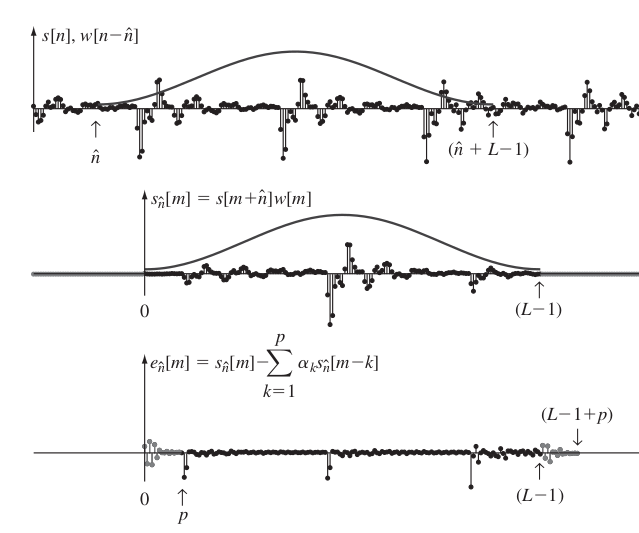
\includegraphics[scale=0.3]{img/hamming.png}
    \caption{Efecto de la ventana de Hamming en los extremos de un frame.}
    \label{fig:hamming}
\end{figure}


